\chapter{GP-EKF: Non-parametric dynamic system using AIS tracking data}\label{chap:gp_ekf}
One of the significant issues with the direct approach is the unimodal assumption of using a \acrshort{gp}. It works well as long as vessels agree on a specific trajectory but fails as soon as there are multiple branching trajectories. A non-parametric dynamical model is proposed in this chapter and used to simulate vessel trajectories to solve this problem. This chapter was inspired by \cite{pedestrian,gpekf,vehicle_gp_prediction}.



The vessel trajectory $\boldsymbol{\mathcal{T}}$ can be expressed using the dynamical system
\begin{subequations}
    \begin{align}
        \boldsymbol{x}_{t+1}       & = \boldsymbol{x}_t + \vec{f}(\boldsymbol{x}_t,\tau_t)\Delta \tau            \\
        \boldsymbol{\mathcal{T}}_t & = \boldsymbol{x}_t + \epsilon, \quad \epsilon \sim \mathcal{N}(0, \sigma^2)
    \end{align}
\end{subequations}
The function $\vec{f}(\cdot): \mathcal{R}^3 \to \mathcal{R}^2$ denotes the vector field describing the expected velocity. In the case of long-term prediction, the dynamics $\vec{f}(\cdot)$ is unknown and is unlikely to be stationary. Instead of using the usual parametric approaches to ODE models, the goal of this chapter is to use a \acrshort{gp} to create a non-parametric representation of the dynamics $\vec{f}(\cdot)$ by learning from historical trajectories of other vessels. This way, arbitrary complex dynamics can be learned without being limited by a fixed parametrization. The \acrshort{gp} considered in this chapter is a vector-valued \acrshort{gp} with zero mean and identical kernel for each output dimension, as expressed in \cref{eq:gp_vec_field}. The output dimensions are assumed to be independent.

\begin{equation}\label{eq:gp_vec_field}
    \vec{f}(\boldsymbol{x}, t) = \vec{f}(\boldsymbol{\eta}) = \begin{bmatrix} f_E (\boldsymbol{\eta})\\ f_N (\boldsymbol{\eta})\end{bmatrix} \sim \text{GP} \big(0 , \; k(\boldsymbol{\eta}, \boldsymbol{\eta}')\big)
\end{equation}

The pipeline for making predictions using available \acrshort{ais} data will now be introduced in greater detail, but can be summarized as:
\begin{enumerate}
    \item Calculate trajectory gradients $\boldsymbol{y}$ for inputs $\boldsymbol{\eta}$ from available \acrshort{ais} data.
    \item Fit a \acrshort{gp} to the time-varying vector-field $\vec{f}: \mathcal{R}^3 \to \mathcal{R}^2$
    \item Simulate the vessel as it is moving through the vector field $\vec{f}$, using either \acrshort{ekf}-based prediction or Sequential Monte Carlo.
\end{enumerate}



\section{Notation and variables}
The key variables for this chapter are summarized in \cref{table:dyngp_key_variables}. All other variables will be introduced as needed.
\begin{table}[h]
    \centering
    \begin{tabular}{ll}
        \textit{\textbf{Variable}}               & \textit{\textbf{Description}}                                      \\ \hline
        $\boldsymbol{x}_t \in \mathcal{R}^2$     & Vessel position at step $t$               \\
        $\tau_t \in \mathcal{R}$                 & Timestamp at step $t$, number of seconds since start of trajectory \\
        $\mathcal{X}_t \in [0, 360)$             & Vessel's course over ground in degrees at step $t$                 \\
        $v_t \in \mathcal{R}$                    & Vessel's speed over ground in knots at step $t$                    \\
        $\boldsymbol{P}_t \in \mathcal{R}^{2x2}$ & State Covariance at step $t$                                       \\
    \end{tabular}
    \caption{Key variables}
    \label{table:dyngp_key_variables}
\end{table}

Note that throughout this chapter, some of the notation used in \cref{sec:gp} will be relaxed in order to reduce the notational complexity. More specifically, the \acrshort{gp}s in this chapter is always assumed to be conditioned on available data, i.e. $p\big(\vec{f}(\boldsymbol{x})\big) = p\big(\vec{f}(\boldsymbol{x}) \; | \; \boldsymbol{y} \big)$.
\section{Method}

The vector-field $\vec{f}$ can be expressed using the \acrshort{gp} framework from \cref{chap:theory} to get the prediction model 
\begin{equation}
    p(\boldsymbol{x}_{t+1} | \boldsymbol{x}_t) = \mathcal{N}\big(\boldsymbol{x}_{t+1} \; | \; (\boldsymbol{x}_t + \mathbb{E}[\vec{f}(\boldsymbol{x_t})] \Delta \tau), (\mathbb{V}[\vec{f}(\boldsymbol{x}_t)] \Delta \tau^2) \big)
\end{equation}

Given a current estimate $p(\boldsymbol{x}_t)$, the marginal next state distribution for the predicted state then becomes 
\begin{equation}
    p(\boldsymbol{x}_{t+1}) = \int_{\boldsymbol{x}_t} p(\boldsymbol{x}_{t+1} | \boldsymbol{x}_t) p(\boldsymbol{x}_t) d\boldsymbol{x}_t
\end{equation} 

However, this integral is intractable, as both the mean and variance depends on the current state $\boldsymbol{x}_t$ with non-trivial relationship \cite{pedestrian,multistep_gp}. One solution to this problem is to use sampling-based methods to numerically approximate this integral. One such approach is proposed later in \cref{sec:dyngp_particle}. Alternatively, the integral can be approximated using a Gaussian distribution. The mean and variance of the Gaussian distribution can be calculated using the law of iterated expecations and conditional variance \cite{multistep_gp}. Assuming the current estimate is distributed according to the Gaussian distribution $p(\boldsymbol{x}_t) = \mathcal{N}(\bar{\boldsymbol{x}}_t, \boldsymbol{P}_t)$, the mean and variance of $\boldsymbol{x}_{t+1}$ is given by

\begin{subequations}
\begin{align}
\begin{split}
    \mathbb{E}[\boldsymbol{x}_{t+1}] &= \mathbb{E}_{\boldsymbol{x}_t}\big[ \mathbb{E}_{\boldsymbol{x}_{t+1}}[\boldsymbol{x}_{t+1} | \boldsymbol{x}_t] \big]\\
    &= \mathbb{E}_{\boldsymbol{x}_t}\big[ \boldsymbol{x}_t + \mathbb{E}_{\vec{f}(\boldsymbol{x}_t)}[\vec{f}(\boldsymbol{x}_t) | \boldsymbol{x}_t] \big]\\
    & = \bar{\boldsymbol{x}}_t + \mathbb{E}_{\boldsymbol{x}_t}\big[ \mathbb{E}_{\vec{f}(\boldsymbol{x}_t)}[\vec{f}(\boldsymbol{x}_t) | \boldsymbol{x}_t] \big]
\end{split}
\end{align}
\begin{align}
    \begin{split}
        \mathbb{V}[\boldsymbol{x}_{t+1}] &= \mathbb{E}_{\boldsymbol{x}_t}\big[\mathbb{V}_{\vec{f}(\boldsymbol{x}_t)}[\vec{f}(\boldsymbol{x}_t) | \boldsymbol{x}_t]\big] + \mathbb{V}_{\boldsymbol{x}_t}\big[ \mathbb{E}_{\vec{f}(\boldsymbol{x}_t)} [f(\boldsymbol{x}_t) | \boldsymbol{x}_t] \big]
    \end{split}
\end{align}
\end{subequations}

The mean and variance of the \acrshort{gp} is the same conditional mean and variance as in \cref{eq:gp_conditional_simple} from \cref{chap:theory}. 


\subsection{EKF trajectory prediction}
Once the dynamics $\vec{f}$ is conditioned on data using \cref{alg:gp_prediction}, it can be used to predict trajectories using the prediction procedure used by the \textit{\acrfull{ekf}}. The combination of \acrshort{gp}s and \acrshort{ekf} was proposed by \cite{gpekf} and is summarized here. The reader is assumed to be already familiar with the Kalman filter and, by extension, the \acrshort{ekf}.

During the prediction procedure, the state is updated incrementally by adding $\vec{f}$ to the current state. In other words, the \acrshort{ekf} prediction model, $g_t(\boldsymbol{x})$, is given by \cref{eq:gp_ekf_prediction}.

\begin{equation}\label{eq:gp_ekf_prediction}
    \hat{\boldsymbol{x}}_{t} = \boldsymbol{g}_t(\boldsymbol{x}_{t-1}) = \boldsymbol{x}_{t-1} + \vec{f}(\boldsymbol{x}_{t-1}, \tau_{t-1})
\end{equation}

Due to the potentially non-linear dynamics of $\vec{f}$, which implies non-linearity in $\boldsymbol{g}(\cdot)$, it is neccessary to linearize the prediction in order to propagate the previous state uncertianty $\boldsymbol{P}_{t-1}$. The Jacobian of the prediction model, $\boldsymbol{G}_t$, is given by \cref{eq:gp_ekf_prediction_jac} where the jacobian of $\vec{f}$ can be computed using \cref{eq:gp_jacobian}. To simplify the notation for the \acrshort{gp} inputs, a new variable $\boldsymbol{\eta} \triangleq \begin{bmatrix}
        \boldsymbol{x} & t
    \end{bmatrix}$ is defined.

\begin{equation}\label{eq:gp_ekf_prediction_jac}
    \boldsymbol{G}_t = \frac{\partial \boldsymbol{g}_t(\boldsymbol{x}_{t-1})}{\partial \boldsymbol{x}_{t-1}} = I + \frac{\partial \vec{f}(\boldsymbol{x}_{t-1}, \tau_t)}{\partial \boldsymbol{x}_{t-1}}
\end{equation}

\begin{align}\label{eq:gp_jacobian}
    \begin{split}
        \frac{\partial \vec{f}(\boldsymbol{x}_*, \tau)}{\partial \boldsymbol{x}_*} &= \frac{\partial \vec{f}(\boldsymbol{\eta})}{\partial \boldsymbol{x}_*} \\  &= \frac{\partial}{\partial \boldsymbol{x}_*} \bigg(\boldsymbol{k}_*^\intercal K^{-1} \big(\boldsymbol{y} - m(X)\big)\bigg)\\
        &= \frac{\partial \boldsymbol{k}_*^\intercal}{\partial \boldsymbol{x}_*} K^{-1} \big(\boldsymbol{y} - m(X)\big)\\
        &= \frac{\partial \boldsymbol{k}_*^\intercal}{\partial \boldsymbol{x}_*} \boldsymbol{\alpha} = \begin{bmatrix}
            \frac{\partial k(\boldsymbol{\eta}_*, \boldsymbol{\eta}_1)}{\partial \boldsymbol{x}_*[1]} & \frac{\partial k(\boldsymbol{\eta}_*, \boldsymbol{\eta}_1)}{\partial \boldsymbol{x}_*[2]} \\
            \frac{\partial k(\boldsymbol{\eta}_*, \boldsymbol{\eta}_2)}{\partial \boldsymbol{x}_*[1]} & \frac{\partial k(\boldsymbol{\eta}_*, \boldsymbol{\eta}_2)}{\partial \boldsymbol{x}_*[2]} \\
            \vdots                                                                                    & \vdots                                                                                    \\
            \frac{\partial k(\boldsymbol{\eta}_*, \boldsymbol{\eta}_N)}{\partial \boldsymbol{x}_*[1]} & \frac{\partial k(\boldsymbol{\eta}_*, \boldsymbol{\eta}_N)}{\partial \boldsymbol{x}_*[2]} \\
        \end{bmatrix}^\intercal \boldsymbol{\alpha}
    \end{split}
\end{align}

The state uncertainty can then be predicted using \cref{eq:gp_ekf_prediction_uncertianty}, propagating the previous uncertainty $\boldsymbol{P}_{t-1}$ using the linearized prediction model $\boldsymbol{G}_t$ and adding the prediction uncertianty $\mathbb{V}[\vec{f}]$.

\begin{equation}\label{eq:gp_ekf_prediction_uncertianty}
    \boldsymbol{P}_t = \boldsymbol{G}_t^\intercal \boldsymbol{P}_{t-1} \boldsymbol{G}_t + \mathbb{V}[\vec{f}(\boldsymbol{x}_{t-1}, \tau_{t-1})]
\end{equation}

The prediction procedure is summarized in \cref{alg:gp_ekf_prediction} and can be used iteratively to simulate a complete trajectory, as demonstrated in \cref{fig:gp_ekf}.

\begin{algorithm}[h]
    \begin{algorithmic}[1]
        \Procedure{GP-EKF-PREDICT}{$\vec{f}$, $\boldsymbol{x}_{t-1}$, $\boldsymbol{P}_{t-1}$, $\Delta \tau$}
        \State $\hat{\boldsymbol{x}}_{t} = \boldsymbol{x}_{t-1} + \mathbb{E}\big[\vec{f}(\boldsymbol{x}_{t-1}, \tau_{t-1})\big] \Delta \tau$
        \State $\boldsymbol{G_t} = I + \frac{\partial \vec{f}(\boldsymbol{x}_{t-1}, \tau_{t-1})}{\partial \boldsymbol{x}_{t-1}} \Delta \tau$
        \State $\hat{\boldsymbol{P}}_t = \boldsymbol{G_t}^\intercal \boldsymbol{P}_{t-1} \boldsymbol{G_t} +\mathbb{V}[\vec{f}(\boldsymbol{x}_{t-1}, \tau_{t-1})] (\Delta \tau)^2$
        \State \textbf{return} $\hat{\boldsymbol{x}}_t, \; \hat{\boldsymbol{P}}_t$
        \EndProcedure
    \end{algorithmic}
    \caption{GP-EKF Trajectory Prediction}
    \label{alg:gp_ekf_prediction}
\end{algorithm}

\begin{figure}
    \centering
    \begin{subfigure}{\textwidth}
        \centering
        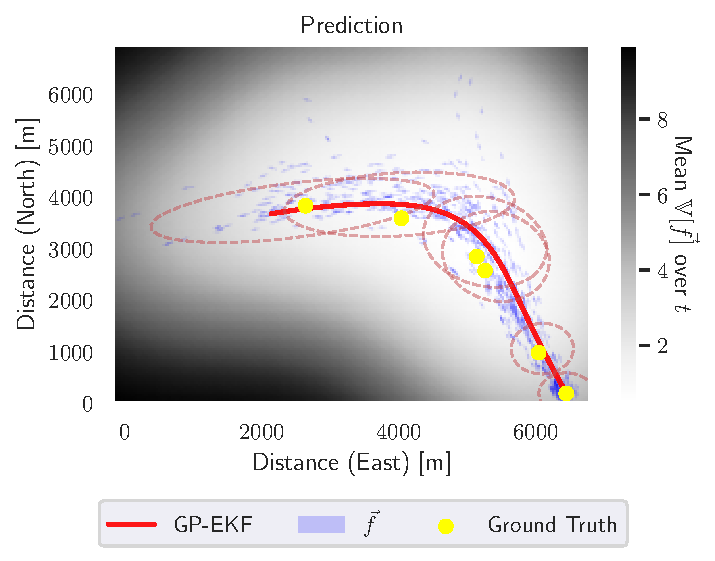
\includegraphics[width=\textwidth]{figures/dyngp/gp_ekf.pdf}
        \caption{Trajectory plotted against the vector-field $\vec{f}(\boldsymbol{x})$. The ellipses show the $95\%$ credibility interval for the predicted trajectory at the ground-truth timestamps.}
    \end{subfigure}
    \begin{subfigure}{\textwidth}
        \centering
        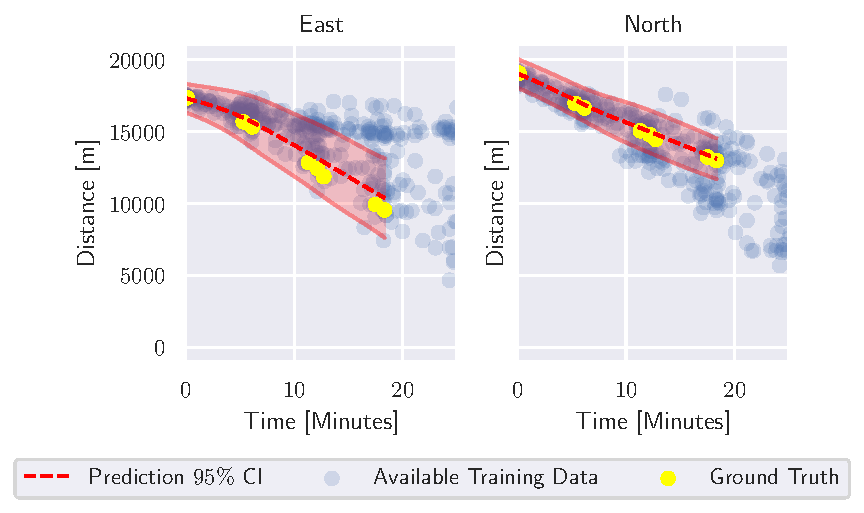
\includegraphics[width=\textwidth]{figures/dyngp/gp_ekf_state.pdf}
        \caption{$95\%$ credibility interval for the trajectory plotted against time}
    \end{subfigure}
    \caption{Predicted position using GP-EKF}
    \label{fig:gp_ekf}
\end{figure}



\subsection{Incorporating vessel position}
While the prediction procedure proposed in \cref{alg:gp_ekf_prediction} yields good predictions in many cases, it is inherently an open-loop prediction. Inaccurate predictions will never be corrected, propagating through any remaining iterations, potentially leading to significant errors later on. \todo[]{Add figure to showcase this issue} It would be desirable if the prediction converged towards available position measurements, \textit{slowly and only if the prediction is clearly wrong}. In other words, weak feedback compensating for minor prediction errors.

As no actual position measurements of the vessel's future position are available, the available training data are considered as \textbf{potential} measurements, which at any timestep may or may not originate from the vessel. Thus, incorporating vessel position becomes a data association problem, for which one can look to target tracking for inspiration.

The \textit{\acrfull{pdaf}} is a method commonly used in target tracking which combines data association and filtering. The following introduction to \acrshort{pdaf} is mostly inspired by \cite{sensorfusjon}, with some adaptations to fit the current problem better. As single target tracking and data association is not the topic of this thesis, only a short introduction to the \acrshort{pdaf} will be included here. For more details, see \cite{sensorfusjon,bar1995multitarget}

In this section, all measurements in the available training set are considered as virtual \footnote{Virtual meaning a measurement that did not actually originate from the target vessel, but rather a measurement that could potentially originate from the target in the future. The word measurement is still used to keep the terminology similar to what is used by \acrshort{pdaf}.} position measurements, which may or may not originate from the vessel at time $t$. Similar to the \acrshort{pdaf}, it is assumed \textbf{at most one} measurement originating from the target to reduce the computational complexity significantly \cite{sensorfusjon}. As there are no proper measurements of the vessel's actual position in the future, most of the measurements are assumed to be clutter, forcing the model to primarily trust its predictions.

Given the predicted state $\hat{\boldsymbol{x}}_t$, any real measurement is expected to be distributed around this state due to some measurement noise. Following the notation used by \acrshort{ekf}, and using the measurement model $h(\boldsymbol{x}) = \boldsymbol{x} \implies H = \frac{\partial h (\boldsymbol{x})}{\partial \boldsymbol{x}} = I$, the predicted measurement distribution is expressed as in \cref{eq:gp_ekf_pdaf_measurement} where the innovation covariance is defined as $\boldsymbol{S}_t \triangleq \hat{\boldsymbol{P}}_t + \boldsymbol{R}$ and $\boldsymbol{R}$ is the measurement noise.

\begin{equation} \label{eq:gp_ekf_pdaf_measurement}
    \hat{\boldsymbol{z}}_t \sim \mathcal{N}(\hat{\boldsymbol{x}}_t, \boldsymbol{S}_{t}) = \mathcal{N}(\hat{\boldsymbol{x}}_t, \hat{\boldsymbol{P}}_t + \boldsymbol{R})
\end{equation}

There is also the possibility that none of the measurements originated from the target, and all observations are clutter. A good clutter model is a complicated topic, but the Poisson clutter model is used in this thesis. As the measurements are not actual measurements from the target, it is difficult to assign meaning to any clutter model. It, therefore, simply boils down to which parameters need to be tuned \footnote{The trajectory prediction is here considered to be target tracking of future position. The clutter parameters, therefore, need to be interpreted in the context of target tracking, not trajectory prediction.} and the Poisson clutter model should already be familiar to anyone with experience in target tracking.
According to the Poisson clutter model, the association probabilities are given by \cref{eq:pdaf_clutter_association_prob} \cite{sensorfusjon}, where $a_t$ is a discrete variable following a Categorical distribution where $a_t=k > 0$ denotes that measurement $k$ originated from the target. $a_t = 0$ is the special case when none of the measurements originated from the target, i.e., the predicted state should not be updated. $Z$ denotes a matrix of all the measurements (positions) available in the training data and is independent of time, i.e., all measurements are always potential candidates. $\lambda$ denotes the clutter rate, and $P_D$ denotes the probability of detecting the target vessel.
\begin{equation}\label{eq:pdaf_clutter_association_prob}
    \Pr\{a_t | Z\} \propto \begin{cases}
        \lambda (1 - P_D)                                                                 & a_t = 0 \\
        P_D \mathcal{N} (\boldsymbol{z}^{a_t} | \hat{\boldsymbol{x}}_t, \boldsymbol{S}_t) & a_t > 0 \\
    \end{cases}
\end{equation}

Using the likelihood for each of the possible outcomes, the association probabilities $\boldsymbol{\beta}$ can be computed by normalizing the likelihood, i.e.

\begin{equation}
    \beta_t^{a_t=i} = \frac{\Pr\{a_t=i \; | \; Z\}}{\sum_{k=0}^M \Pr\{a_t=k \; | \; Z\}}
\end{equation}

The predicted state can then by updated using the Kalman update procedure for each the measurements individually. As the measurements $\boldsymbol{z}_t^{a_t > 0}$ are known values, the state innovation $\boldsymbol{v}_t^{a_t>0} \triangleq \boldsymbol{z}_t^{a_t>0} - \hat{\boldsymbol{z}}_t$ is distributed according to the measurement prediction $\hat{\boldsymbol{z}}_t$.

\begin{equation}
    \boldsymbol{v}_t^{a_t>0} \sim \mathcal{N}(\boldsymbol{z}_t^{a_t>0} - \hat{\boldsymbol{x}}_t, S_t)
\end{equation}
The updated state for each measurement is then given by the normal \acrshort{ekf} update step

\begin{subequations}
    \begin{align}
        \boldsymbol{x}_t^{a_t > 0} & = \hat{\boldsymbol{x}}_t + \boldsymbol{W}_t \boldsymbol{v}_t^{a_t > 0} \\
        \boldsymbol{P}_t^{a_t > 0} & = \ (\boldsymbol{I} - \boldsymbol{W}_t) \hat{\boldsymbol{P}}_t
    \end{align}
\end{subequations}
where $\boldsymbol{W}_t \triangleq \hat{\boldsymbol{P}}_t \boldsymbol{S}_t^{-1}$ is the Kalman gain.
The updated state of the vessel over all possible measurements can be described as a Gaussian Mixture Model over the $M+1$ different modes weighted by the association probabilites, i.e.
\begin{equation}
    p(\boldsymbol{x_t}) = \underbrace{\beta_t^{a_t=0} \mathcal{N}(\boldsymbol{x}_t \; | \; \hat{\boldsymbol{x}}_t, \hat{\boldsymbol{P}}_t)}_{\text{No measurements are valid}} + \sum_{k=1}^M \underbrace{\beta_t^{a_t=k} \mathcal{N}\big(\boldsymbol{x}_t | \boldsymbol{x}_t^{a_t=k}, \boldsymbol{P}_t^{a_t=k}\big)}_{\text{Measurement $k$ is valid}}
\end{equation}


Moment reduction is then used to combined the different hypothesises into a single unimodal Gaussian distribution, i.e. a Gaussian distribution is fitted to the first and second moment (mean and variance) of the Gaussian mixture. The mean and variance of the resulting distribution is given by \cref{eq:pdaf_moment_mean} and \cref{eq:pdaf_moment_var} respectively, using $\boldsymbol{v}_t \triangleq \sum_{a_t > 0} \beta_t^{a_t} \boldsymbol{v}_t^{a_t}$.

\begin{subequations}
    \begin{align}
        \boldsymbol{x}_t & = \hat{\boldsymbol{x}}_t + \boldsymbol{W}_t \boldsymbol{v}_t \label{eq:pdaf_moment_mean} \\
        \begin{split}
            \boldsymbol{P}_t &= \hat{\boldsymbol{P}}_t - (1 - \beta_t^{0}) \boldsymbol{W}_t \boldsymbol{S}_t  \boldsymbol{W}_t\\ &+ \boldsymbol{W}_t \big[\sum_{a_t > 0}^M \beta_t^{a_t} \boldsymbol{v}_t^{a_t} (\boldsymbol{v}_t^{a_t})^\intercal - \boldsymbol{v}_t \boldsymbol{v}_t^\intercal \big] \boldsymbol{W}_t^\intercal\label{eq:pdaf_moment_var}
        \end{split}
    \end{align}
\end{subequations}

While available measurement could be used at each timestep, it is in practice more convenient only to include a subset that is close enough to the predicted state. As this measurement \textit{gate} should scale with the uncertainty, the gated subset is selected as \cref{eq:pdaf_gate} where $g$ is the number of standard deviations the method should consider.

\begin{equation} \label{eq:pdaf_gate}
    \mathcal{G} = \big\{ \boldsymbol{z}^{a_t > 0} \; | \; (\boldsymbol{z}^{a_t > 0} - \hat{\boldsymbol{x}}_t)^\intercal S^{-1} (\boldsymbol{z}^{a_t > 0} - \hat{\boldsymbol{x}}_t) < g^2 \big\}
\end{equation}


By combining the \acrshort{pdaf} update with the GP-EKF prediction procedure in \cref{alg:gp_ekf_prediction}, the predicted trajectory can be tuned to favor areas with a large number of samples, effectively pulling the state towards areas with available samples. Conversely, in regions with samples spread evenly around the predicted state, then the \acrshort{pdaf}'s effect is negligible (assuming proper tuning).

However, the \acrshort{pdaf} has severe impacts on the state uncertainty, as the update procedure causes an unwanted reduction in uncertainty. The effect can, to some extent, be tuned using $\mathbf{R}$, but it then becomes a tradeoff between a too low gain $\boldsymbol{W}$ and an overconfident $\boldsymbol{P}$. In other words, the \acrshort{pdaf} update either has no effect on the state or becomes overconfident. Furthermore, as this is a pure prediction method and the measurements are not originating from the target, it is unrealistic to expect the uncertainty to reduce over time. Hence, the GP-EKF prediction is a more realistic representation of the true uncertainty. Ideally, the state should be updated using the \acrshort{pdaf} procedure without affecting the uncertainty. While not elegant, a quick and dirty solution to this is to omit the uncertainty update in \cref{eq:pdaf_moment_var}. The predicted state is then pulled toward the measurements without affecting the uncertainty. There is no mathematical justification for doing this, but it is found to give the desired behavior. This concludes the development of the modified{\footnote{It is called the \textbf{modified} \acrshort{pdaf} update because the state covariance is not updated.}} \acrshort{pdaf} update, which is summarized in \cref{alg:gp_ekf_pdaf}.

\begin{algorithm}[h]
    \begin{algorithmic}[1]
        \Procedure{GP-EKF-MODIFIED-PDAF}{$\hat{\boldsymbol{x}}_{t}$, $\hat{\boldsymbol{P}}_{t}$, | $\mathbf{R}$, $\lambda$, $p_D$, $g$}
        \State $\boldsymbol{S}_t = \hat{\boldsymbol{P}}_t + \boldsymbol{R}$ \Comment{Innovation Covariance}
        \State $\boldsymbol{W}_t = \hat{\boldsymbol{P}}_t \boldsymbol{S}_t^{-1}$\Comment{Kalman Gain}
        \For{each measurement $\boldsymbol{z}^{a_t > 0}$}
        \State $\boldsymbol{v}_t^{a_t>0} = \boldsymbol{z}^{a_t>0} - \hat{\boldsymbol{x}}_t$ \Comment{Innovation}
        \State $\tilde{\beta}^{a_t>0} = \mathcal{N}(\boldsymbol{v}_t^{a_t > 0} \; | \; 0, \boldsymbol{S}_t)$ \Comment{Unnormalized Weight}
        \EndFor
        \State $\tilde{\beta}_t^{a_t = 0} = \lambda (1-p_D)$ \Comment{Unnormalized Clutter Probability}
        \State $\boldsymbol{\beta} = \frac{\tilde{\boldsymbol{\beta}}}{\sum_{a_t} \tilde{\beta}^{a_t}}$ \Comment{Normalize weights}
        \State $\boldsymbol{x}_t = \hat{\boldsymbol{x}}_t + \boldsymbol{W}_t \big(\sum_{a_t > 0} \beta^{a_t} \boldsymbol{v}_t^{a_t} \big)$\Comment{Update the state mean}


        \State \textbf{return} $\boldsymbol{x}_t, \; \hat{\boldsymbol{P}}_t$
        \EndProcedure
    \end{algorithmic}
    \caption{GP-EKF Modified \acrshort{pdaf} update}
    \label{alg:gp_ekf_pdaf}
\end{algorithm}


\begin{figure}
    \centering
    \begin{subfigure}{\textwidth}
        \centering
        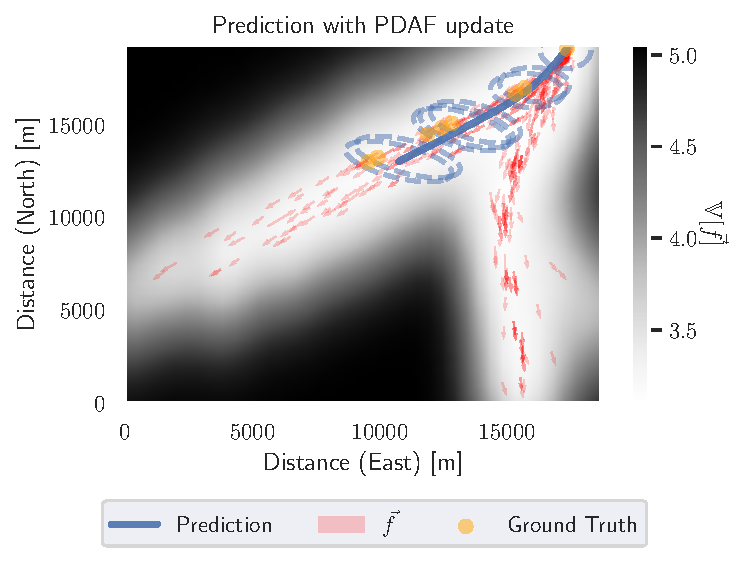
\includegraphics[width=\textwidth]{figures/dyngp/gp_ekf_with_pdaf.pdf}
        \caption{Trajectory plotted against the vector-field $\vec{f}(\boldsymbol{x})$. The ellipses show the $95\%$ credibility interval for the predicted trajectory at the ground-truth timestamps.}
    \end{subfigure}
    \begin{subfigure}{\textwidth}
        \centering
        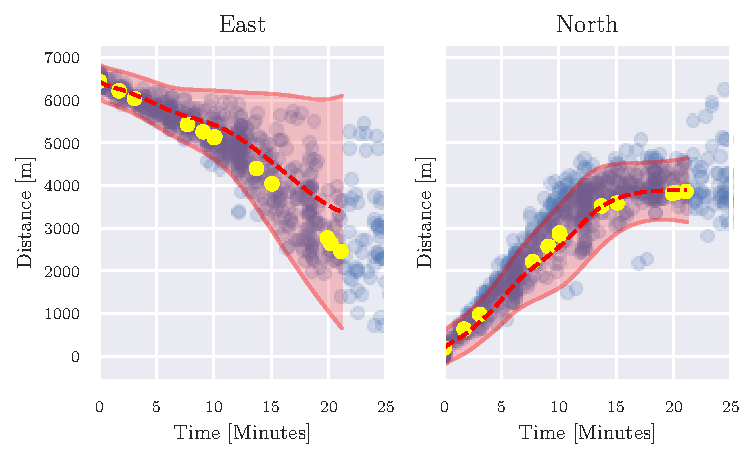
\includegraphics[width=\textwidth]{figures/dyngp/gp_ekf_with_pdaf_state.pdf}
        \caption{$95\%$ credibility interval for the trajectory plotted against time}
    \end{subfigure}
    \caption{Predicted position with the PDAF update procedure.}
    \label{fig:gp_ekf_with_pdaf}
\end{figure}

\subsubsection{Tuning PDAF parameters}
The model should primarily trust the prediction model, as it would get stuck as the measurements do not change over time. If the \acrshort{pdaf} parameters are tuned too aggressively, it tends to affect the velocity estimates of the prediction negatively. In practice, it has worked well tuning the measurement noise $\boldsymbol{R}$ to get the desired update effect.
However, finding a set of parameters that works well across different trajectories turns out to be challenging. Parameters that improve the prediction for one trajectory may do more harm than good on another. The performance of using PDAF will be explored further in \cref{chap:stat_testing}.

\subsection{Simulating trajectories using Gaussian Process Sequential Monte Carlo}\label{sec:dyngp_particle}
The Kalman-based prediction scheme proposed in the previous section works well as long as a single Gaussian distribution can sufficiently explain the uncertainty. However, in branching trajectories, minor differences in position early in the predicted trajectory might significantly affect the following predictions. The result is a multimodal trajectory distribution, which a Kalman-based approach is not able to express.

Inspired by the prediction step used by \textit{particle filters} \cite{sensorfusjon}, the idea of sampling trajectories can be used to explore the multimodal trajectory distribution. While inspired by the particle filter, this approach will from now on be referred to as \textit{Sequential Monte-Carlo} to avoid confusion\footnote{a vital part of the particle filter is weighting the particles based on available measurements. As only the sampling of trajectories is performed, Sequential Monte-Carlo seems like a better fit.}, as well as to follow the same naming convention as used by \citeauthor{pedestrian} \cite{pedestrian}.

The derivation of the Sequential Monte-Carlo approach is embarrassingly simple as this method trades high computational complexity for more straightforward mathematics. Instead of analytical propagation of uncertainty, many trajectories are simulated through random sampling and used to express the uncertainty empirically. As a result, the uncertainty for any trajectory distribution can be described, though at the cost of considerable computational complexity.
$N$ different trajectories are initialized with similar initial conditions. The trajectories are then simulated by drawing independent increments from $\vec{f}$ using the approach described in \cref{sec:gp_samples}, conditioned on the current state of each trajectory. The result is visualized in \cref{fig:gp_particle} for $N=500$ trajectories.
\begin{figure}[h]
    \centering
    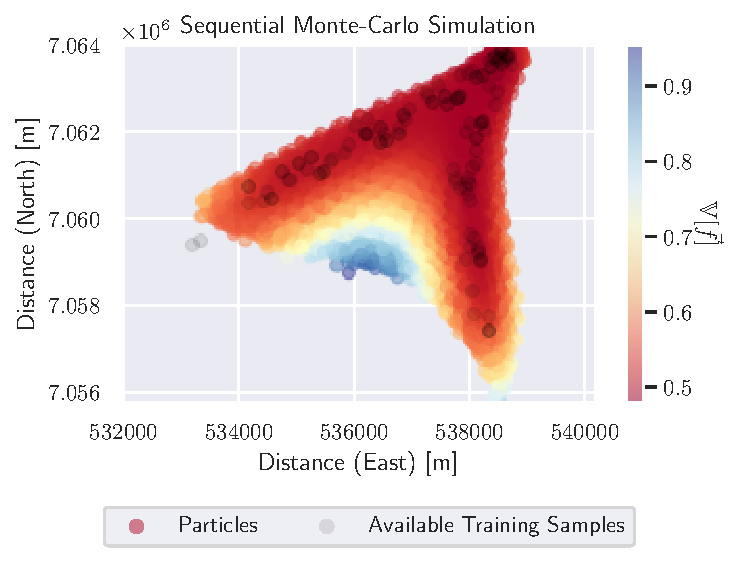
\includegraphics[width=\textwidth]{figures/dyngp/gp_particle.pdf}
    \caption{}
    \label{fig:gp_particle}
\end{figure}

\subsection{Training Source}
There are two potential sources for the training samples $\boldsymbol{y}$:

\begin{enumerate}
    \item Trajectories from the dataset are converted into training samples for $\vec{f}$ using the simple first-order finite-difference method in \cref{eq:finite_difference} between subsequent \acrshort{ais} samples in a trajectory $i$. This yields the training outputs $\boldsymbol{y}_t^{i}$ corresponding to the inputs $\boldsymbol{\eta}_t^i$ such that $\boldsymbol{y}_t^i = \vec{f}(\boldsymbol{\eta}_t^i) + \epsilon$.
    \item The \acrshort{cog} and \acrshort{cog} from the \acrshort{ais} data can be used directly.
\end{enumerate}

\begin{align}\label{eq:finite_difference}
    \boldsymbol{y}_t = \frac{\boldsymbol{x}_{t+1} - \boldsymbol{x}_t}{\tau_{t+1} - \tau_t}
\end{align}


However, in practice, the dataset contains several contradicting trajectories. For example, in a given area, vessels may move in opposite directions or with vastly different speeds. Therefore, the data is clustered based on the trajectories' initial conditions, and the appropriate cluster for prediction is selected using the target vessel's current position, \acrshort{cog} and \acrshort{sog}. A straightforward pipeline is used in this thesis to cluster relevant trajectories for training, given the vessel's current state. Note that this is the same pipeline used in \cref{chap:direct_gp}, but is restated here for completeness.

\begin{enumerate}
    \item The initial position of the trajectory must be close to the queried position $\boldsymbol{x}_0$. In this thesis, a fixed threshold $\Delta \boldsymbol{x}$ is used.
    \item The initial \acrshort{cog} must be close to the queried heading $\mathcal{X}_0$. In this thesis, a fixed threshold $\Delta \mathcal{X}$ is used.
    \item The initial \acrshort{sog} must be close to the queried velocity $v_0$. In this thesis, a fixed threshold $\Delta v$ is used.
    \item If there are more than $N$ samples in the training set, then the samples are picked from the trajectories with the closest initial position.
\end{enumerate}

\section{Choice of kernel}
Finding a good kernel that works well across different situations is a tricky task. The \acrshort{rbf} is a safe choice, which works well in most cases, as long as the trajectories are reasonably smooth. This makes the simple \acrshort{rbf} the go-to kernel in this thesis.

A possible extension is to use the sum of two \acrshort{rbf} kernels to get some additional flexibility. This kernel in \cref{eq:gp_ekf_kernel} attempts to model the data as a combination of a long-term trend, dependent noise, and independent noise. This is the same kernel proposed in \cref{chap:direct_gp}, though without the \acrshort{cog} and \acrshort{sog} input dimensions. It works better than the \acrshort{rbf} kernel in some of the more complicated cases, though at the cost of more hyperparameters to tune. In simple cases, hyperparameter optimization typically reduces the scale parameter $\sigma_1$ such that the dependent noise kernel $k_1$ has a negligible effect.

\begin{equation}\label{eq:gp_ekf_kernel}
    k(\boldsymbol{\eta}_i, \boldsymbol{\eta}_j) = \sigma_0 k_0(\boldsymbol{\eta}_i, \boldsymbol{\eta}_j) + \sigma_1 k_1(\boldsymbol{\eta}_i, \boldsymbol{\eta}_j) +  \sigma_2 \delta(i, j)
\end{equation}

\begin{description}
    \item[Long term trend $k_0$] is a \acrshort{rbf} kernel intended to cover the long-term behavior of the trajectories, i.e., a smooth component describing the overall trend of the trajectories. The lengthscales of this kernel are assumed to be large.
    \item[Dependent noise $k_1$] is a \acrshort{rbf} kernel intended to model the variability between different trajectories not well explained by $k_0$. The lengthscales are assumed to be short.
    \item[Independent noise $\delta(i, j)$] is a white kernel intended to model any remaining error as \acrshort{iid}.
\end{description}

Several other kernels were also attempted, though no statistical testing was performed. A few notable experiments:
\begin{description}
    \item[Matern + White] The Matern class of kernels were attempted with $\nu=0.5$, $\nu=1.5$ and $\nu=2.5$. None of these gave any improved performance and the $\nu=0.5$ at times caused optimization errors.
    \item[\acrshort{rbf} + Matern + White] was tried with $\nu=\frac{1}{2}$, $\nu=\frac{3}{2}$ and $\nu=\frac{5}{2}$ without showing any benefits over the simpler \acrshort{rbf} based kernel in \cref{eq:gp_ekf_kernel}.
    \item[\acrshort{rbf} + Rational-Quadratic + White] The Rational Quadratic kernel was attempted as a replacement for the \acrshort{rbf} kernel as the dependent noise. No improvements was found, so the simpler \acrshort{rbf} was preferred.
\end{description}


\subsection{Optimizing the hyperparameters}
The hyperparameters can be optimized using the \acrshort{ml} approach discussed in \cref{sec:gp_mle}.

The whole dataset cannot be used to find the optimal hyperparameters due to the computational complexity. Two approaches are proposed to mitigate this issue:
\begin{enumerate}
    \item Fit the hyperparameter to many different subsets of the available training data and use the median values. The median is preferred over the mean values to avoid issues with outlier parameter estimates. This approach tends to find a set of hyperparameters that work well across a wide range of cases but may become too general for challenging scenarios.
    \item Rerun the hyperparameter optimization for each scenario. This approach tends to find the optimal parameters in each case. However, it is also error-prone as it is not guaranteed to find a global optimum, and it may cause overfitting.
\end{enumerate}

The first approach is preferred in most cases, as it finds a global set of parameters and tends to result in smoother functions $\vec{f}$.


\section{Summary}
This chapter has so far introduced a lot of new concepts, so that it might be nice with a summary of the overall pipeline:

\begin{enumerate}
    \item Based on the target vessel's current state, such as position, \acrshort{cog} and \acrshort{sog}, trajectories with similar initial conditions is selected from the training set.
    \item Training inputs $\boldsymbol{\eta}$ and outputs $\boldsymbol{y}$ for $\vec{f}$ are generated from the training trajectories.
    \item The kernel hyperparameters are optimized using \acrshort{ml} to find the parameters which best explains the training data. This is either done once to find a global set of parameters or individually for each scenario.
    \item The training data and kernel can then used to get the conditional distribution for $\vec{f}$.
    \item The \acrshort{ekf} procedure in \cref{alg:gp_ekf_prediction} is called repeatedly, using the current state of the target vessel as initial conditions. At each step, the \acrshort{pdaf} update procedure can be used as well if desired. Sequential Monte-Carlo can alternatively be used to simulate multimodal trajectories.
\end{enumerate}

The only parameters which need manual tuning are the time increment $\Delta \tau$ and the initial covariance $\boldsymbol{P}_0$. All other parameters are learned from the data.
